\justifying
As discussed in the main text, the GO solution was prepared using a modified Hummers' method\cite{Hummers1958} with additional pre-processing of the graphite powder.\cite{Kovtyukhova1999} The preoxidation of the graphite powder (5 g; d $= 45\ \mu$m) was completed using sulfuric acid (30 mL; 97\% H$_{2}$SO$_{4}$), phosphorus pentoxide (4.2 g; P$_{2}$O$_{5}$), and potassium persulfate (4.2 g; K$_{2}$S$_{2}$O$_{8}$) in a water bath at 75$^{\circ}$C for 4.5 h. The mixture was then cooled to room temperature and diluted with 700 mL of deionized water (DI) and vacuum filtered through a poly(tetrafluoroethylene) membrane (pore size $5\ \mu$m). After pre-oxidation, the graphite was subjected to a modified Hummers' method.\cite{Hummers1958} During this process, the pre-oxidized material was suspended in H$_{2}$SO$_{4}$ (150 mL; 97\%) in an ice bath for 20 min. Potassium permanganate was slowly added (15 g; KMnO$_{4}$) and the mixture was heated to 35 $^{\circ}$C for 2 h. Hummers' method was completed by adding 250 mL of DI water and heating the mixture to 70$^{\circ}$C for an additional 2 h. After quenching the reaction with hydrogen peroxide (30 mL; H$_{2}$O$_{2}$) and DI water (750 mL), it was allowed to cool to room temperature. In order to quench the unreacted reagent and clean the solution, the product was then filtered through a 300 $\mu$m testing sieve, then through glass fiber and centrifuged for 2 h at 5000 RPM (\textit{Sorvall RC-5C} plus). The supernatant was then washed with hydrochloric acid (400 mL, 10\% HCl). The sieving, centrifugation, and washing process was then repeated using DI (two times) and ethanol (EtOH, two times). The final solution was then dispersed in 300 mL of EtOH at a concentration of $\approx 0.1$ wt\%.

%\section{Graphene Oxide Nanoscroll Formation}

Various stages of the formation of three different GONS are displayed in Fig.~\ref{figS1_AppB}. In Fig.~\ref{figS1_AppB}a a large portion of the GO sheet has not scrolled, indicating an early stage of GONS formation. Fig.~\ref{figS1_AppB}b is GONS in a more advanced state, in which the majority of the GO sheet is scrolled around the main structure. Fig.~\ref{figS1_AppB}c is near the end of the formation of GONS as characterized by an almost complete scrolling of the GO.

\begin{figure}[h!]
 \centering
 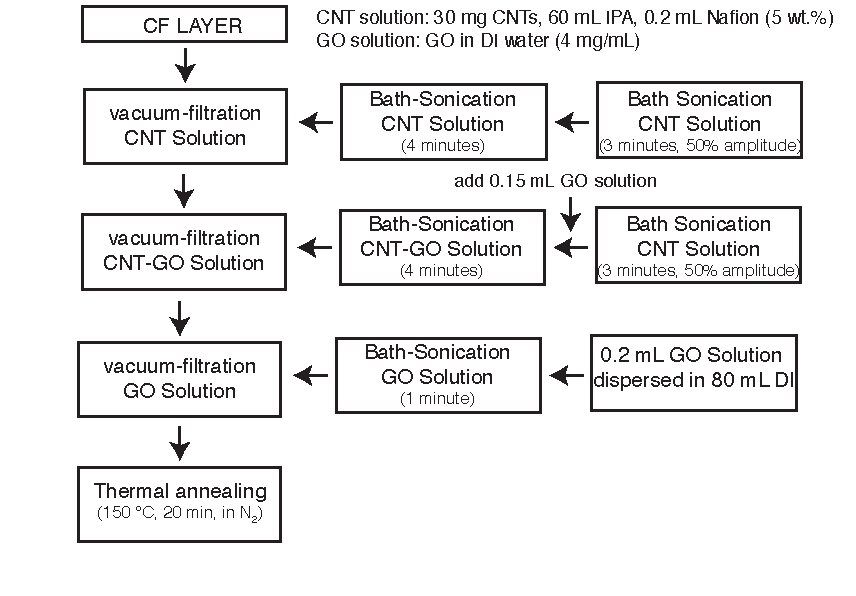
\includegraphics[height=5in]{FigS1.pdf}
  \caption{\textbf{Different stages of GONS formation.} \textbf{(a)} Early stage formation. \textbf{(b)} Advanced stage formation. \textbf{(c)} Final stage formation.}
  \label{figS1_AppB}
\end{figure}

\newpage

The different geometries depicted in Fig.~3 in the main text can originate from the same GO flake. Fig.~\ref{figSa_AppB} represents a scrolled GO flake where it is possible to recognize two T-GONS and one C-GONS.

\begin{figure}[h!]
  \centering
  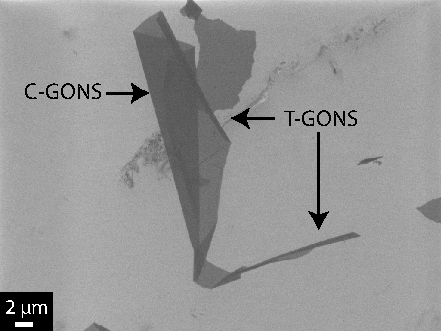
\includegraphics{FigSa.pdf}
  \caption{\textbf{Formation of a scrolled GO flake displaying simultaneously T-and C-GONS.}}
  \label{figSa_AppB}
\end{figure}
%\newpage

Fig.~\ref{figSa_AppB} demonstrates the hollow nature of the GONS acquired \textit{via} transmission electron microscopy. Fig.~\ref{figSa_AppB}a presents GONS whose tail (right side) is not scrolled in accordance with the multi-layer structure. Fig.~\ref{figSa_AppB}b presents open-structure GONS, characteristic of an incomplete scrolling process.

\begin{figure}[h!]
  \centering
  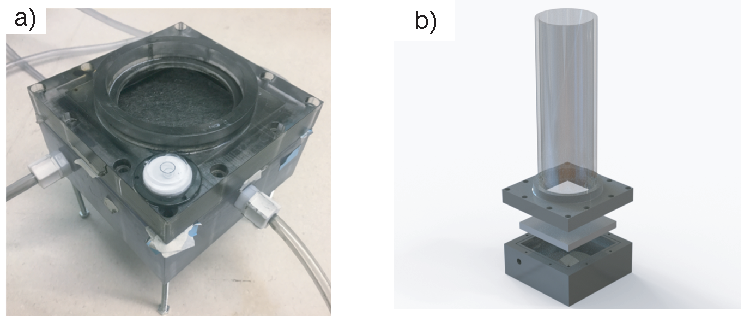
\includegraphics[width=5in]{FigS2.pdf}
  \caption{\textbf{Transmission electron microscopy (TEM) of GONS.} \textbf{(a)} TEM image of GONS with a defective (wrinkled) tail. \textbf{(b)} TEM image of open-structure GONS formed by partial scrolling.}
  \label{figS2_AppB}
\end{figure}

\newpage

Fig.~\ref{figS4_AppB} represent the statistical analysis of the GONS diameters for different geometries. Statistical data is based on a population of $10-15$ GONS for each geometry. Fitting with normal distributions shows that the diameter of the narrow tube-like GONS is $225 \pm 85$ nm ($\mathbb{R}^{2} = 0.9964$) while the diameter of the wide tube-like GONS is $1.802 \pm 0.273\ \mu$m ($\mathbb{R}^{2} = 0.99$). Also, the Gaussian fits show that the minimum diameters of the cone-like GONS are $193 \pm 1$ nm ($\mathbb{R}^{2} = 0.9999$) for the narrow cone and $0.948 \pm 0.317\ \mu$m ($\mathbb{R}^{2} = 0.8722$) for the wide cone, while the maximum diameters are $1.65 \pm 0.391\ \mu$m ($\mathbb{R}^{2} = 0.9668$) for the narrow cone and $1.84 \pm 0.331\ \mu$m ($\mathbb{R}^{2} = 0.9548$) for the wide cone.

\begin{figure}[t!]
  \centering
  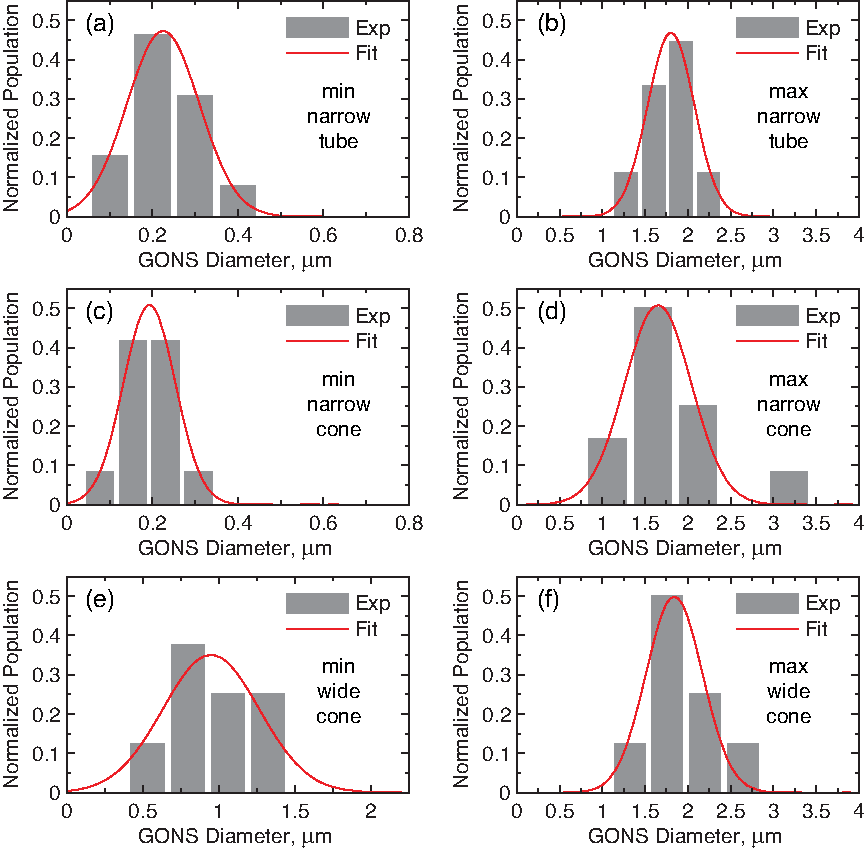
\includegraphics[height=5in]{FigS3.pdf}
  \caption{\textbf{Histograms of the GONS diameters and normal distribution.} \textbf{(a)} Diameter distribution for narrow tube GONS. \textbf{(b)} Diameter distribution for wide tube GONS. \textbf{(c)} Minimum diameter distribution for narrow cone GONS. \textbf{(d)} Maximum diameter distribution for narrow cone GONS. \textbf{(e)} Minimum diameter distribution for wide cone GONS. \textbf{(f)} Maximum diameter distribution for wide cone GONS.}
  \label{figS4_AppB}
\end{figure}

\clearpage

Fig.~\ref{figS5_AppB} represents an AFM image of GONS. The cross-section line highlights its multilayered structure. On the left side of the image, it is possible to notice a GO flake not wrapped around the GONS characterized by a thickness of $\approx2$ nm. The GONS maximum thickness is $\approx12$ nm and it displays a noticeable wrinkle on the outer most layer.

\begin{figure}[h!]
  \centering
  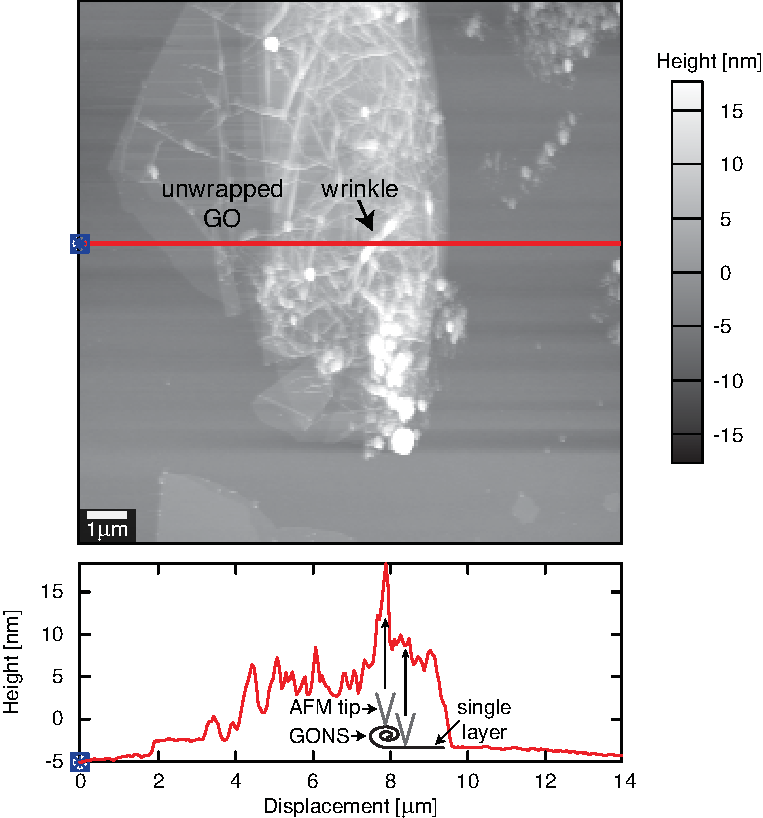
\includegraphics[width=3.5in]{FigS4.pdf}
  \caption{\textbf{AFM image of GONS and cross-section line that illustrates its multilayer structure.}}
  \label{figS5_AppB}
\end{figure}

\clearpage

Fig.~\ref{figS6_AppB} represents the C1s peak for the parent GO flake (Fig.~\ref{figS6_AppB}a), after 5 minutes of LF irradiation (Fig.~\ref{figS6_AppB}b), and 5 minutes of HF irradiation time (Fig.~\ref{figS6_AppB}c). The post-treatment XPS shows a reduction in the C-O peak from 65\% to $\approx25\%$, and increase in C-C/C=C from 30\% to $\approx60\%$ which is related to the cleavage of GO sheet at oxygen defects in the basal plane as explained in the main text.

\begin{figure}[h!]
  \centering
  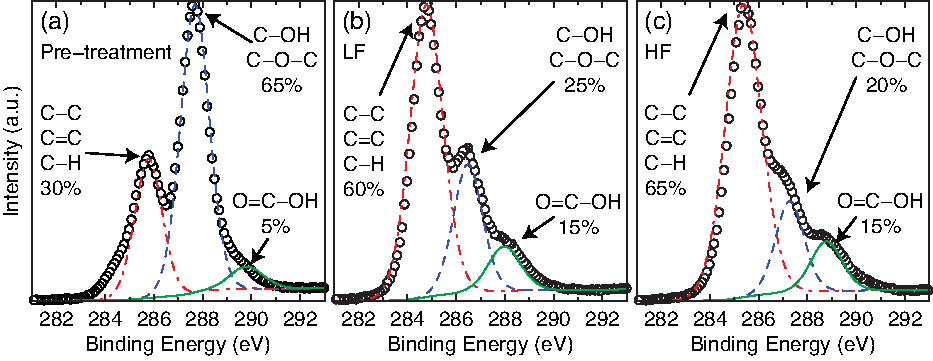
\includegraphics{FigS6.pdf}
  \caption{\textbf{XPS before and after ultrasonic treatment.} \textbf{(a)} XPS pre-treatment. \textbf{(b)} XPS after 5 min ultrasonic treatment at low frequency (LF). \textbf{(c)} XPS after 5 min ultrasonic treatment at high frequency (HF).}
  \label{figS6_AppB}
\end{figure}

\newpage
%\section{Graphene Oxide Flake and Nanoscroll Dimension Scaling}

%\subsection{Image Analysis}

\begin{figure}[h!]
  \centering
  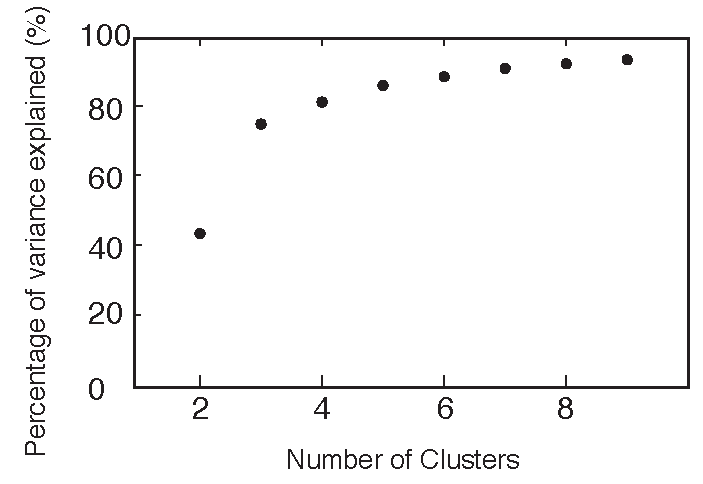
\includegraphics[width=4in]{FigS5.pdf}
  \caption{\textbf{Picture taken from the built-in color threshold function of \textit{ImageJ} used for analyzing the GO flake area.}}
  \label{figS7_AppB}
\end{figure}

Fig.~\ref{figS7_AppB} represents an SEM image analyzed by \textit{ImageJ} in order to determine the size distribution of the GO flake. The statistical analysis is based on 300 GO flakes taken from 5 different SEM images for each processing time.

\clearpage

%\subsection{Scaling Relations}

Table~\ref{tblS1_AppB} and Table~\ref{tblS2_AppB} present the experimental data for the GO flake area ($A_{\mathrm{GO}}$) and the length of the produced GONS ($L_{\mathrm{GONS}}$). See Fig.~4 and Fig.~5 in the main text for plots.

\begin{table}[h]
 \begin{center}
 \caption{\textbf{Experimental data for the evolution of the GO flake area ($A_{\mathrm{GO}}$) as a function of the treatment time ($t$) for both the low frequency (LF) and high frequency (HF) treatments.} The values reported are the mean values and their standard errors.}
  \label{tblS1_AppB}
  \begin{tabular}{c|c|c|c|c|c}
        \hline
         t & HF(1 W) & HF(10 W) & HF(20 W) & LF(10 W) & LF(100 W) \\
         $[$min$]$ & $A_{\mathrm{GO}}$ [$\mu$m$^{2}$] & $A_{\mathrm{GO}}$ [$\mu$m$^{2}$] & $A_{\mathrm{GO}}$ [$\mu$m$^{2}$] & $A_{\mathrm{GO}}$ [$\mu$m$^{2}$] & $A_{\mathrm{GO}}$ [$\mu$m$^{2}$] \\
        \hline
        0 & $52.8 \pm 3.9$ & $52.8 \pm 3.9$ & $52.8 \pm 3.9$ & $52.8 \pm 3.9$ & $52.8 \pm 3.9$ \\
        5 & $53.4 \pm 6.4$ & $44.4 \pm 4.9$ & $45.5\pm 1.8$ & $17.3 \pm 1.1$ & $3.7 \pm 0.1$ \\
        10 & $51.0 \pm 4.5$ & $39.5 \pm 3.0$ & $25.7 \pm 1.5$ & $9.8 \pm 1.0$ & $3.5 \pm 0.4$ \\
        20 & $57.1 \pm 5.9$ & $30.8 \pm 2.4$ & $13.3 \pm 1.2$ & $10.6 \pm 0.7$ & $2.7 \pm 0.2$ \\
        30 & $47.5 \pm 5.2$ & $26.0 \pm 1.5$ & $16.1 \pm 1.1$ & $8.1 \pm 0.7$ & $2.0 \pm 0.2$ \\
        60 & $51.3 \pm 4.2$ & $31.9 \pm 1.7$ & $14.6 \pm 0.9$ & $6.7 \pm 0.7$ & $1.7 \pm 0.2$ \\
        \hline
  \end{tabular}
 \end{center}
\end{table}

\begin{table}[h]
 \begin{center}
 \caption{\textbf{Experimental data for the evolution of the GONS length ($L_{\mathrm{GONS}}$) as a function of the treatment time ($t$) for both the low frequency (LF) and high frequency (HF) treatments.} The values reported are the mean values and their standard errors.}
  \label{tblS2_AppB}
  \begin{tabular}{c|c|c|c|c|c}
        \hline
         t & HF(1 W) & HF(10 W) & HF(20 W) & LF(10 W) & LF(100 W) \\
         $[$min$]$ & $L_{\mathrm{GONS}}$ [$\mu$m] & $L_{\mathrm{GONS}}$ [$\mu$m] & $L_{\mathrm{GONS}}$ [$\mu$m] & $L_{\mathrm{GONS}}$ [$\mu$m] & $L_{\mathrm{GONS}}$ [$\mu$m] \\
        \hline
        5 & $10.3 \pm 1.2$ & $11.3 \pm 1.2$ & $10.9\pm 1.8$ & $6.8 \pm 0.8$ & $2.5 \pm 0.4$  \\
        10 & $9.2 \pm 0.8$ & $8.3 \pm 0.8$ & $8.2 \pm 1.5$ & $5.7 \pm 0.6$ & $2.3 \pm 0.4$ \\
        20 & $8.7 \pm 1.0$ & $6.5 \pm 0.5$ & $7.2 \pm 1.2$ & $5.4 \pm 0.5$ & $1.4 \pm 0.2$ \\
        30 & $9.0 \pm 0.8$ & $6.5 \pm 0.6$ & $7.2 \pm 1.1$ & $3.8 \pm 0.6$ & $1.0 \pm 0.1$ \\
        60 & $10.0 \pm 1.0$ & $6.8 \pm 0.6$ & $7.2 \pm 0.9$ & $2.8 \pm 0.2$ & $1.0 \pm 0.1$ \\
        \hline
  \end{tabular}
 \end{center}
\end{table}

\clearpage

%\subsection{Solution Volume Dependence}

\begin{figure}[htp]
  \centering
  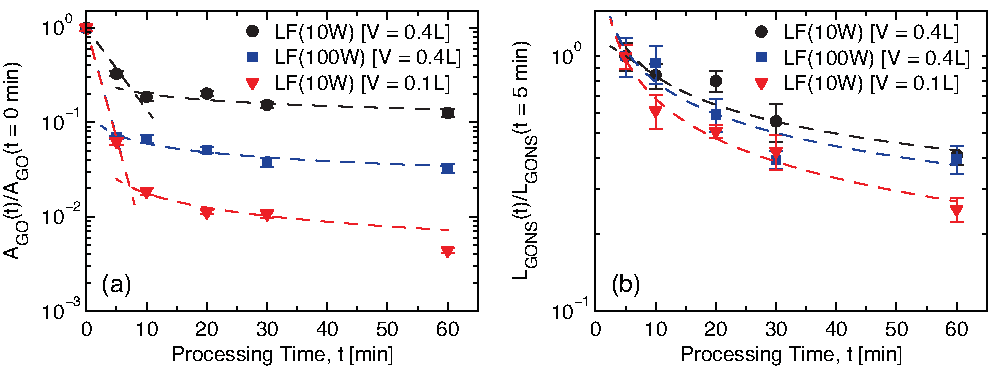
\includegraphics[width=6.5in]{FigSb_rev2.pdf}
  \caption{\textbf{Influence of the solution volume ($V$) on the evolution of $A_{\mathrm{GO}}$ and $L_{\mathrm{GONS}}$ as a function of the treatment time ($t$).}}
  \label{figSb_AppB}
\end{figure}

Since the volume of the GO solution used during HF and LF processing could affect the $A_{\mathrm{GO}}$ and $L_{\mathrm{GONS}}$, but this effect will be more pronounced in the highly destructive LF treatment method, and may alter the $A_{\mathrm{GO}}$ and $L_{\mathrm{GONS}}$ evolution kinetics presented in Eq. 1 and Eq. 2 in the main text. As Fig.~\ref{figSb_AppB} illustrates, reducing the volume of the solution used in the LF(10W) treatment leads to a faster reduction in $A_{\mathrm{GO}}$ ($A_{1} = 101.7\ \mu$m$^{2}$, $k_{\mathrm{GO}} = 0.538$, $A_{2} = 5.99\ \mu$m$^{2}$, $s_{1} = 0.50$, and $t_{\mathrm{crit}} = 7.1$ min) and $L_{\mathrm{GONS}}$ ($L_{2} = 5.1\  \mu$m, $s_{2} = 0.518$,  and $t_{\mathrm{crit}} \leq 5$ min), but the general kinetics are very similar to the ones observed for LF(100W) and are consistent with Eq. 1 and Eq. 2 in the main text.
